\documentclass[10pt]{article}
\usepackage{titling}
\usepackage[margin=0.75in]{geometry}
\usepackage{graphicx}
\graphicspath{ {images/} }

\title{Winter Progress Report}
\author{
	Dylan Davis, Trevor Hammock, Alex Schultz \\
    Group 18 \\
	Oregon State University\\
	Corvallis, Oregon
}
\date{\today}

\begin{document}
\begin{titlingpage}
\maketitle

\begin{abstract}
This document serves to inform all interested parties of the progress made on the HP Big Data Analytics project as of February 21st, 2018; a week-by-week synopsis details what we individually achieved. Additionally, project purposes, goals, problems, and our achievements are discussed.
\end{abstract}
\end{titlingpage}


\tableofcontents
\clearpage

\section{Project Purposes and Goals}
PageWide Web Press, a printing division within HP, produces and supports industrial digital web presses. All of the web presses currently deployed  in the market generate product data, which the PageWide Web Press team receives on a daily basis. The data is eventually stored into a Oracle Database and is used to perform business analytics and resolve issues with the web presses.

The large amount of data created some issues for the division; on average, they receive around 350GB of product data per day, which generates Database tables with billions of rows. This massive influx of data has stressed the division's storage and performance capabilities of their current hardware. The current, non-optimized environment, significantly increases the amount time it takes to process and analyze that data, and the division wants to find a more efficient data storage solution. Furthermore, the amount of data that is received everyday has slowly been increasing over time. The current rate of 350GB of data per day will increase, so preparation and efficiency are essential.

If nothing is done about the data collection process, the division may need to make a costly investment into better hardware that satisfies their growing storage and performance needs. Alternatively, they may have to invest into big data software platforms, like Hadoop, that are more optimized and scalable for their given workloads. This project will address the aforementioned issues by using system enabled compression to reduce the amount of physical space that the data occupies. The overall goal for this project is to research system enabled compression options that are available to Oracle Databases and see how these options affect physical storage and query performance. Knowledge obtained from research will be used to accurately predict and measure the way in which data is inserted and stored in the Oracle database.

\section{Week by Week Synopsis}
\subsection{Alex Schultz}

\subsubsection{Winter Break}
At the end of Fall term, Kirby and Andy wanted us to look into data blocks a little further in order to determine how data is stored in a block. Their reasoning for the investigation is to deduce how compression affects the size of the data. Additionally, if we were able to figure out how data is stored in a block, we would be able to finish our equation, which will allow us to accurately calculate how much data can fit in a block without running any queries or even starting up the database. Although we were set to meet on December 20th 2017, I was unable to attend due to illness. I then started working full time at my job, preventing me from attending the meeting on January 3rd 2018. I did read over my teammate's notes and familiarized myself with their progress so that I did not fall behind. As a result, I was up to speed when we met for the first time Winter term.

\subsubsection{Week One}
The first ten minutes of the meeting were spent bringing one of our clients up to speed, as he was also unable to attend on December 20th 2017 and January 3rd 2018. Once everyone was on the same page, we read over the client's outline for the Oracle Hotsos presentation. Having understood the direction of the presentation, we were asked to create a set of slides that succinctly describe how block compression works. We were to use simple language that everyone can understand, yet provide enough detail to convey relevance; the Oracle conference will include highly technical people, after all. These slides are important because they will aid in the client's success during their presentation; it is imperative to ensure the audience can easily follow them so that significant points are understood. We also discussed and created the tests we wanted to run that would reveal the best method of optimizing the client's environment. 

The student team congregated 4 times outside of the normal weekly meeting to ensure goals were met punctually. During these meetings we discussed the most efficient methods of measuring data in addition to starting and finishing the slide show presentation. My portion of the presentation included providing pictures and a description of how columns are reordered at the block level. I described how columns are reordered based on cardinality, and how Oracle stores columns from low to high cardinality. The more unique data in a column, such as an email address, the higher the cardinality. Oracle's method allows the most duplicated data to appear first within a block, which makes it quicker when querying data. Furthermore, I researched CPU and IO diagnostic tools that are compatible with Oracle databases. Some possibilities were SQLd360, SQL Tuning Advisor, and Oracle Enterprise Manager.

\subsubsection{Week Two}
We presented the slide show that we created and the client provided insight as to how we can improve. Having generated the test data in week one, we were ready to begin testing query performance on the test tables. In terms of performance, our client was most interested in CPU usage and Input/Output (IO) due to their prominent influence on query performance. An important aspect of testing query performance is deciding which tool to use. We know we wanted the most accurate data, so the team collectively searched for the best tool to use. Eventually the client decided to use Snapper, a tool developed by Tanel Poder, which pulls data directly from Oracle. The client then asked us to become familiar with Snapper and ensure it is effective. Additionally, we were to expand upon our slides by introducing pictures to supplement the text. 

\subsubsection{Week Three}
I was able to run Snapper successfully, and did not have any issues doing so. I think this was because I took some time to watch Tanel Poder's two videos on it. My teammates asked me to create a short tutorial explaining how I used it, so I created a two minute video explaining what to do from start to finish. Unfortunately, I found it difficult to export Snapper data into a CSV because Oracle was running in a virtual machine where I did not have Excel. However, I personally found that Snapper gathered data relevant to our needs, and the team concurred. Snapper became our official tool to analyze our test suite. To validate our test results, the client asked us to individually run all the tests and compare results to see how they vary across hardware. I ran the tests, analyzed the results, and summarized my findings for the client.

\subsubsection{Week Four}
Week four introduced the first assignments in CS462: the progress report, presentation, and the poster. As the team captain, I began by reading over the requirements and started mapping out what needed to be done and by what time. At that point it was sufficient to simply advise my teammates that we had deliverables assigned. I also started thinking about the 30 second to 1 minute pitches we could give at the expo in Spring. 

Our client had to cancel our meeting; however, we were able to reschedule a couple days later. This was a very important meeting because we discovered that our methodology was not sound - we used insufficiently sized tables and had multiple variables that prevented us from recording accurate results. As a group we decided to concoct new tests, which maintain the 800 to 1 parent/child ratio, yet introduced a ten-fold increase in table size. I, along with my teammates, ran the new test suite and began to analyze the results and summarize discoveries. 

\subsubsection{Week Five}
I wanted to get a head start on the poster because it was due in the middle of week 6, so I looked at the requirements and downloaded the template from the College of Engineering page. I then simply read the template and thought about what we could put on the poster and where it would go.

Due to unforeseen meetings, the client was not able to attend our scheduled meeting for week 5. Lack of availability between the team and the client prevented a rescheduled meeting. Fortunately, we are not a complacent team. We continued to run more experiments that tested CPU and IO performance across the 8 tables. I ended up graphing Trevor's data, which was astounding because he controlled for external variables and maintained a minimal standard deviation. These Excel charts, we agreed, were going to be very useful in conveying the differences between each test and table. 

\subsubsection{Week Six}
We knew that we had to deliver the poster, report, and presentation this week, so those were our top priorities outside of attending the meeting with our client. We successfully finished the poster in one sitting, making sure to satisfy all the requirements. We also began working on the presentation slides, which we used as a template for the report.

Despite not meeting during week 5, I don't feel like we lost any momentum. We presented our results to the client and he looked at the charts I made in week 5. He was happy with our results, but there were two loose ends. One is that the sorted tables use significantly less CPU than random tables, and the second is that normalized tables are faster than denormalized tables. Our new objective is to find out why, and one of the client's suggestions was to create a flame graph, which visually details the Oracle database call stack trace. As soon as we are able to determine why sorted is better than random with respect to CPU, and why normalized tables are faster than denormalized tables, then we will have effectively and successfully completed the capstone research project. 

\subsection{Dylan Davis}

\subsubsection{Winter Break}
During winter break, our team continued to meet at HP and research Oracle compression. This was our last 
chance to learn as much as we could about how the compression algorithm and the database itself work as we 
planned to begin running our actual experiments in January. To make sure we had the most time possible, we met 
each Wednesday of the break except for the week of Christmas. Our most important discoveries over the break were 
how binary dumps of rows are encoded so Oracle knows the difference between tokens and uncompressed columns as 
well as more information about how multi-column tokens and rows with multiple tokens work.

Oracle stores bytes in the binary dump of each row that represent which data from the token table belongs in the 
row or that represent the length of the next column value in bytes if the data is stored in the row itself. Our 
goal during winter break was to figure out how Oracle distinguishes between a byte representing a token and a 
byte representing a column length as well as how it handles token values and column lengths that would require 
more than one byte to represent. This would allow us to understand the decisions Oracle made when compressing 
data so that we could more easily calculate the compression ratio for specific data by hand without actually 
using the database. From our previous study of data blocks, we noticed that token values in the binary dump 
always started at 00 and went up from there, whereas column lengths always started at C9, or 201 in hexadecimal, 
for columns with a length of one byte and went up from there. We decided to create some test tables that 
would result in more than 256 tokens and tables that had column values lengths of greater than 256 bytes. What 
we found was that token values greater than 199 and column lengths greater than 50 were represented by a string 
of three bytes. A column length in this range started with a hexadecimal FA and then used the other two bytes to 
give the length of the column in bytes. A token in this range followed a similar pattern but instead starts 
with an FB. We also found that null column values not at the end of a row are represented with an FF while null 
values at the end of a row are not stored in the binary dump. The last single byte token, token 199, is 
represented by C7 while the single byte column length, 50 bytes, is represented by F9. C8 and FC through FE are 
most likely used for special cases, although we were not able to create a situation where they were used. 

These findings answered both of our questions about token and column length bytes. Using the encoding described 
above, Oracle can represent smaller token and column length values with a single byte while also being able to 
represent larger values easily with three bytes. This encoding also removes any ambiguity from the binary dump. 
Oracle can tell if a byte is a token or a column length simply from its value. This also allows us to predict 
exactly how many bytes will be needed to store a compressed data block.

A final important discovery we made over winter break was that tokens can be made up of any combination of other 
tokens and raw data and that tokens do not all have to appear at the beginning of a row but can instead be 
scattered throughout. 

\subsubsection{Week One}
Our first priority for week one was to go over the progress we had made so far, make sure everyone was up to 
speed, and make a plan for the following two months before the HotSOS convention. We went over this in our first 
meeting of winter term. Kirby then went over the scripts he had created for us to run to create the data tables 
we would be performing experiments on. He designed these tables to somewhat reflect the actual data stored in 
HP's database. These tables had a wide range of ratios between parent and child tables, were either compressed 
or uncompressed, and were in either random or sorted order. There were also pre-combined parent/child tables, 
some as normalized tables and others as denormalized. All tables used either 8K, 16K, or 32K block sizes. We 
also made plans to begin creating presentation slides to explain our findings throughout this research project. 

After our first meeting, we each ran these table creation scripts on our own machines to create our test data. 
We then studied various meta data about the tables, including overall size, number of blocks, rows per block, and 
number of tokens used per block. Each of us also began work on the presentation slides mentioned above. 

\subsubsection{Week Two}
During our meeting in week two, we studied our findings from running Kirby's table creation script. We found 
that sorted, compressed tables had many more rows per block than unsorted, compressed tables. This was due to 
the fact that their are fewer repeating values but many more instances of the few repeating values in a single 
block of a sorted table, which meant the token table was much smaller and each token in it represented many more 
values within the table. This left more room for actual table rows within the block. Normalized tables were also 
much smaller in size because much of their data was represented by keys that corresponded to a row in one of 
several reference tables we created. These normalized tables were then compressed and made even smaller. 

During this meeting, we also went over the presentation slides we had created so far and discussed what needed 
to be more concise and what needed to be expanded upon. 

Finally, we discussed options for tools we could use to gather CPU and I/O data while running our test queries 
on our data tables. After going over several available data collection tools, we decided to use Snapper, which 
is a script that runs in the background and collects data from several of the database views while a query is 
performed. 

During this week, we began to familiarize ourselves with the Snapper tool. After running several tests, we 
learned how to run the script and how to most efficiently collect the outputted data and store it in easily 
viewable files. We also continued our work on our presentation slides.

\subsubsection{Week Three}
During this weeks meeting, our main focus was to decide on the best queries to run on our test data tables to 
gather CPU and I/O stats. We wanted to run queries that would join the parent and child tables and also have to 
perform a mathematical operation on some of the data and group the data by certain columns as this would reflect 
more closely a typical query of HP's actual database. Eventually, we settled on the query we would use for the 
separated parent and child tables. However, we still had not finalized our queries for the combined normalized 
and denormalized data tables and would need to write these on our own time. Once we had decided on our query, 
we also began practicing running snapper to gather stats about that query. 

Outside of our meeting, we came up with the queries to run on the combined normalized and denormalized tables. 
We ran these by Kirby to be sure we would be getting the kinds of results he was looking for and he approved 
them. Over the course of the week, each of us ran our selected queries while running Snapper on our own machines 
and collected and saved the resulting data to be analyzed fully during our next meeting. 

\subsubsection{Week Four}
This week, our meeting had to be rescheduled to Friday. During the meeting we went over our data gathered from 
Snapper while running our queries. While some findings were useful, we decided that, to reduce the effect of 
CPU noise on our findings, we should create tables of ten million rows rather than one million. 
We selected only eight of the most interesting tables, based on our findings so far, for which to create
ten million row versions. Also, we discussed ways we could prevent caching of data from affecting our results. 

Over the following weekend, we wrote the script to create the ten million row tables that were similar in 
structure to Kirby's original tables. We then began using the same queires on these tables while running snapper 
to gather more useful CPU and I/O data. 

\subsubsection{Week Five}
Our week five meeting had to be cancelled due to scheduling conflicts with Kirby and Andy. However, we continued 
collecting CPU and I/O data and sending it to them on our own time. By discusses our experimental procedure and 
findings with each other, we were able to find the best way to gather and organize our data and be sure it 
contained the smallest margin of error possible on our machines. 

This week, we also attended our capstone class period and went over our Expo presentations. 

\subsubsection{Week Six}
During the meeting of week six, we went over our collected data on queries of the ten million row tables. The 
two most important findings that stood out to all of us were, first, that sorted tables were much more 
efficient with regard to CPU than random tables with the same data and, second, that normalized tables were much 
more efficient, also with regards to CPU, than denormalized tables even though they had to perform several joins 
after being decompressed in order to bring in the actual data stored within the reference tables. We viewed 
the execution plans of some of these queires within SQL Developer to try to figure out what might be causing 
these results. 

We then discussed using flame graphs to try to illustrate how exactly Oracle was performing these queires to see 
if that could shed some more light on the findings we made. Also, in order to be sure that the difference in 
efficiency between sorted and random tables did not have to do with compression and token table size, we made 
plans to create sorted and random uncompressed tables and see if the sorted tables still had an advantage. 
Finally, discussed creating two tables, both of equal width, but with one having a very wide repeating value 
column of cardinality 100 and a small random character column, while the other has a small width repeating 
value column, also of cardinality 100, and a very wide random character column. Each table would also have a 
number column that is the same width in each table. We could then query each table, grouping by the repeating 
column and averaging the number column, in order to see if the width of the column being grouped by affects 
CPU efficiency even though the whole table has to be read. This could help us to understand why the normalized 
table, which has smaller width columns, is more efficient than the denormalized table. 

During the rest of this week, we studied how to create flame graphs on our own and practiced making them on our 
own machines. We also created the two varying column width tables to run efficiency tests on. However, we still 
need to run the actual tests on these tables. 

\subsection{Trevor Hammock}

\subsubsection{Winter Break}
Over the break, the team was tasked with investigating how data gets stored in a block. Once this is known, we could come up with an equation that predicts how much data can be jammed within that block. This will ultimately give our team insights into how compression effects the size of the data. To figure this out we first had to solve the mystery of multi-byte tokens and lengths. During Fall term through some unofficial documentation we learned that Oracle uses a single byte to represent tokens and lengths. This can place physical limits on the data within that block because you can only store up to 256 unique values within a single byte. However their is official documentation that defines those limits to be much higher than the single byte limitations, on top of hinting at the existence of multi-byte representations. To answer this I first created a test table that would generate over 256 tokens. Sure enough it was successful but the hexadecimal encoding for that byte left me pondered.

The threshold for the multi-byte tokens was the magic number '0xC7' which means you could have up to 200 tokens before Oracle started using multiple bytes. Me and my team members discussed this and came up with a hypothesis that the column length and token reference were stored within the same byte, meaning that all of the values above the magic number were being used for the column length. I was then tasked with creating a test table that would have row data with column lengths greater than 50. 50 was used because it was what we estimated the remaining address space to be for the column length. Just as we predicted, the threshold for multi-byte length was 50 and confirmed that everything was being encoded in a single byte.

Once this was known we were then on the verge of discovering how Oracle encodes/decodes row data within a block. If we could determine this, then we would essentially have the algorithm to calculate how much data can be stored within a block irregardless if its compressed or uncompressed. To figure this out I located more Oracle documentation that provided some details on how to estimate how much data is stored within a block. Using some hand crafted test data and some additional findings from my peer, Dylan, I was finally able to crack the code and reversed engineered the data storing algorithm.

\subsubsection{Week One}
At the start of the term me and my fellow teammates reported back to our client and went over everything we discovered over the break. We were then individually tasked with making a PowerPoint that discussed our findings that our client would later use for his Hotsos presentation. We then divied up the work and began working on the slides.

We also discussed and designed a suite of tests that we would experiment on. These experiments would prove, or disprove, our findings from our research using real world data. The tables were modeled after our clients current data warehouse environment and would hopefully provide direct insights into how our client could optimize his given environment. Once this was established we then each individually manufactured the test data. We then spent our time doing table size analysis to see if we could draw any conclusions from table compression. To visualize these conclusions I went and created graphs for all of the of situations our client wanted to analyze.

\subsubsection{Week Two}
Now that we had generated the test data and performed all of the size analysis, our next task was to test query performance on the tables. To do this we would need to engineer SQL queries that would stress the tables for their worst case scenario (full table scans). We would also need to come up with a means to measure query performance in Oracle. We knew early on we wanted to measure CPU and IO statistics because this is what ultimately effects query performance for SQL Databases. However the challenge was finding some Oracle Database based tool that could gather this information within a reasonable amount of accuracy and precision. My team and our client looked at a wide range of available tools but ultimately decided that the tool, Snapper, would be the tool that we would use. Our task was to first get the tool up and running, then play with it using some pre-testing, see what kind data it generates, and determine if it is acceptable for our benchmarking needs. With the help of my teammates I eventually got the tool up and running on my system but I was only able to do a minimum amount of pre-testing.

\subsubsection{Week Three}
Our team reconvened with our client and unanimously decided to use the tool for our benchmarking needs. This was due to the simplicity of the tool and fairly accurate data it was able to provide. We then agreed upon a test suite of queries that we wanted to run and each individually collected our own set of data. This was so we could gather data from a wider range of hardware so we would not bias our conclusions on an individual machine, this is primarily due to different hardware having its own unique set of bottlenecks that could effect query performance. On my own I was able to run the test suite and gather all of the necessary data. I then started to analyze the data and started to draw conclusions that I would later report to our client.

\subsubsection{Week Four}
My team and our client met once again and we went over the experiments we were suppose to run. We also discussed our individual results and the conclusions we were able to draw from them. Unfortunately, we didn't realize it but my team originally had a lot of flaws in our testing methodology. This was a culmination of many factors which included insufficient table size, inconsistent testing practices, and inability to reduce the noise in our experiments. To alleviate this we decided to run a new set of tests with a refined set of testing methodology to be able to collect a better set data. Since we were able to draw some conclusions from the results, we were able to remove some of the tests from our testing suite to primarily focus on the table configurations that showed promise. I then set out to run our new test suite and gathered a fairly sizable amount of data. Once that was done I then spent a fair chunk of time analyzing and drawing conclusions from all of the data we gathered from this new round of testing.

\subsubsection{Week Five}
We were originally scheduled to meet with our client this week and discuss our data and findings. Unfortunately, our client got caught up in a lot meetings and we were unable to reschedule a meeting for this week. So as a team we continued to collect even more data which would allow us to refine and solidify the conclusions that we would end up making about our experiments. Just like last week, I collected a fair amount of data and also spent most of my time analyzing all of the data that my team collected for the week.

\subsubsection{Week Six}
My team then met up with our client and discussed our findings. He was very pleased with the data and most of the results backed up our predictions. However their were two anomalies in the data that we were unable to explain. We were then individually tasked with investigating those anomalies on our own time. I decided to investigate why the sorted tables happen to use significantly less CPU. It was expected to use less CPU but it was unexpected to make a significant difference (we observed a 23\% to 26\% improvement). I decided to create two equally sized uncompressed tables with similar data where one was sorted and the other was not. Interestingly even though the tables were of equal size and uncompressed, the sorted version still showed a 24\% improvement. One of my fellow teammates, Dylan, also performed a similar set of tests and was also able to generate the same exact results. Next I decided to generate flame graphs as a means to analyze the call stack of our Database instance from the operating system's perspective. If the Database happens to use different calls, varying amounts of those calls, with variable processing times then the flame graph will make those differences very obvious. I was able to generate the graphs, however I encountered a fair bit of noise due to how I was collecting the data. I will continue to generate the flame graphs and see if I can refine my testing methodology to minimize the amount of noise from the data.


\section{Current progress}
Fall term was a great success, in that the team was able to successfully reverse engineer Oracle data blocks and the Oracle Basic Compression algorithm. These breakthroughs allowed the team to make educated hypotheses, given certain data/table sets, as to what would happen with data size, compression, and tokens. During the first 6 weeks of Winter term, the team formed well-constructed experiments that provided insight as to how certain queries are affected with respect to query performance, CPU usage, disk IO, and time. We created 8 tables with which to test: 8K uncompressed, 8K random, 8K sorted, 8K parent join child, 8K parent join child normalized, 32K sorted, 32K parent join child, and 32K parent join child normalized. Database CPU, CPU used by the session, SQL execute elapsed time, database time, file IO wait time, user IO wait time, and direct path read all served as metrics, which we graphed in the figures below. Our current and final task is to discern why sorted tables have a better effect on CPU than random tables, and why normalized tables are faster than denormalized tables.

\section{Charts}
The first chart displays each table with respect to CPU used by the Oracle database session. We clearly see that 32K Parent/Child Normalized produces the best results. However, it is unconventional to use 32K block sizes, so the most appropriate conclusion is that 8K Parent/Child Normalized tables produce the best results with respect to CPU. \newline \newline
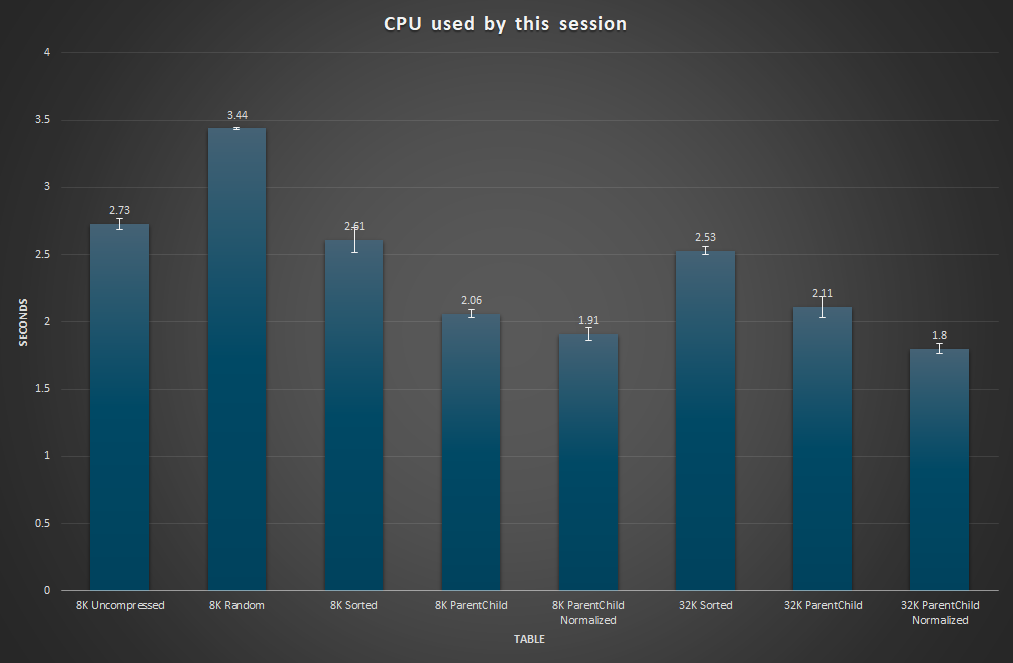
\includegraphics[scale=0.5]{cpu.png} \newline \newline
The second chart reveals file IO wait time differences between each of the 8 test tables. We notice that 8K Sorted yields the best results due to the unconventional use of 32K block sizes. \newline \newline
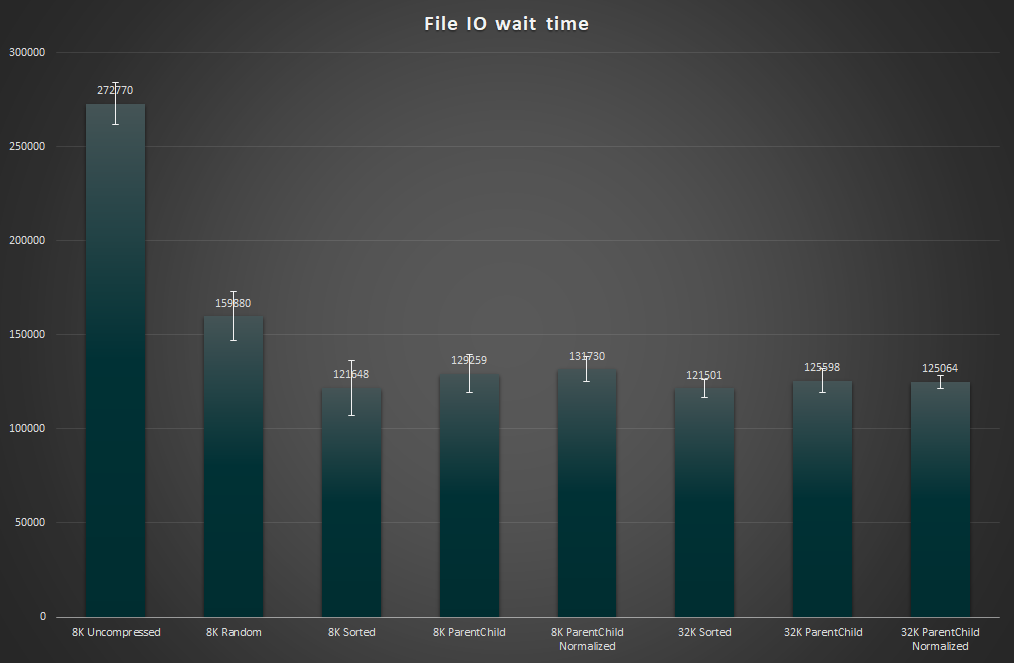
\includegraphics[scale=0.5]{file_io.png}

\section{Problems and Solutions}
We have a rock solid team; therefore, we encountered no problems amongst ourselves. The only problems we encountered were cancelled meetings and an insufficient methodology when running our tests. We were able to reschedule all meetings except one, and we quickly rectified our methodology within a week. Despite the research-oriented project, each milestone was met punctually.

\section{Conclusion}
Fall term was used to familiarize the team with basic concepts and environment configuration. Winter term concluded the research project as we developed our test suite, ran experiments, and analyzed the data to recognize a conclusion. Future work potentially includes investigating network compression, index compression, and whatever else the client may want to pursue.

\end{document}